\documentclass[11pt]{article}

\usepackage[utf8]{inputenc}

\usepackage[T1]{fontenc}

\usepackage[margin=1in]{geometry}

\usepackage{graphicx}

\usepackage[hidelinks]{hyperref}

\graphicspath{{figures/}}

\setlength{\parindent}{0pt}

\setlength{\parskip}{0.45em}

\title{GRNScope: a web server for transparent multi-method gene regulatory network inference from single-cell data}

\author{Author details to be supplied}

\date{15 October 2026}

\begin{document}

\maketitle

\begin{center}\small\emph{Working draft; public URL and validation study pending.}\end{center}

\begin{abstract}

Gene regulatory network (GRN) inference from single-cell expression data is sensitive to algorithm choice, preprocessing and sampling variation. Comparing methods often requires separate software environments and manual reconciliation of outputs with different score scales. GRNScope is a web application that validates expression matrices, runs multiple GRN inference methods in isolated environments and presents their results through an interactive network, edge table, trajectory and method-comparison views. It reports per-target rank evidence separately from recovery across cell-bootstrap replicates and from agreement among methods. We demonstrate the implemented workflow using the 19-gene, 2,000-cell BEELINE gonadal sex determination example, with supplied pseudotime. All 13 selected methods completed; the automatic repeat-run procedure completed three to seven bootstrap replicates per method. Median pairwise Spearman correlation between replicate rankings varied from 0.415 to 0.999 across methods, exposing differences in repeat-run stability that are hidden by a single network output. The demonstration has no uploaded reference network and does not establish biological accuracy. GRNScope makes computational evidence and its limits inspectable while preserving method-specific outputs for further analysis. \textbf{Public server URL: [to be supplied before submission].}

\end{abstract}

\textbf{Keywords:} single-cell RNA-seq; gene regulatory networks; web server; reproducibility; method comparison

\section{Introduction}

GRNs provide a framework for describing candidate relationships between regulators and target genes. Single-cell RNA sequencing supplies variation across cells from which these relationships can be inferred, but expression association alone does not establish direct or causal regulation. Methods also differ in whether they use static expression, pseudotime or external priors, and in whether they predict direction or regulatory sign. These differences complicate interpretation of any one inferred network.

BEELINE brought a diverse set of GRN inference methods into a common benchmarking framework and showed that their behaviour depends on the dataset and evaluation criterion \cite{pratapa2020}. The underlying algorithms remain useful in their own right: PIDC uses multivariate information measures \cite{chan2017}, GENIE3 uses tree-based prediction \cite{huynhthu2010}, and GRNBoost2 offers a scalable boosting-based approach \cite{moerman2019}. For researchers using several methods, however, preparing compatible inputs, managing software dependencies and comparing heterogeneous ranked outputs still impose practical costs. A web interface can reduce those costs if it preserves the distinctions among evidence, repeatability and biological validation.

GRNScope makes three specific contributions to the practical use and interpretation of existing GRN inference methods. First, it provides a single workflow for validating inputs, recording preprocessing choices and executing methods in separate software environments. Second, it presents three distinct forms of computational evidence without combining them into a single accuracy claim: per-target edge ranks show priority within a method, cell-bootstrap recovery shows sensitivity to resampling, and between-method comparisons show overlap among predictions. Third, its interactive result views and exports preserve method-specific information, including the number of returned edges and whether a method can infer direction or regulatory sign. Together, these features let users trace a displayed relationship back to the method output and examine how consistently it was recovered. Here we describe the implementation and a completed example analysis, then identify the further comparisons and biological evidence needed to evaluate predictive accuracy.

\section{Server and analysis workflow}

\subsection{Inputs, preprocessing and execution}

The principal input is a delimited expression matrix with genes as rows and cells as columns. Optional files provide pseudotime, cluster labels, a reference network or other method-specific information. GRNScope validates identifiers and numeric content before starting an analysis, then presents the inferred matrix state and preprocessing choices to the user. In the present demonstration, the uploaded matrix was recorded as log-normalized; no additional normalization or logarithmic transformation was applied. A detection filter required expression in at least 10\% of the 2,000 cells, equivalent to 200 cells, and retained all 19 genes (Fig. 1).

The Next.js/React frontend communicates with a FastAPI backend. Selected algorithms execute as separate jobs in isolated computational environments. The project stores the uploaded and processed files, resolved parameters, per-method results and run metadata. Users can inspect a method's results while other methods continue. The completed project analysed here selected PEARSON, PPCOR, SINCERITIES, CellOracle, PIDC, LEAP, GRNBoost2, SCRIBE, GRISLI, GENIE3, SINGE, SCODE and GRNVBEM. Pseudotime was supplied with the input rather than estimated by this run. CellOracle uses prior-informed network modelling \cite{kamimoto2023}; its outputs should therefore be interpreted alongside, rather than treated as directly interchangeable with, methods without the same prior requirements.

\subsection{Evidence and repeat-run confidence}

Raw scores from different algorithms are not pooled because their scales and meanings differ. For each target gene within one method, GRNScope ranks unique candidate regulators by the absolute value of the method's score, assigning average ranks to exact ties. If an edge has rank \(r\) among \(R\) candidates for that target, its normalized rank evidence is \(E=1-(r-1)/(R-1)\) when \(R>1\), and \(E=1\) when there is only one candidate. This is a within-method, within-target ordering measure, not a probability of physical regulation.

Each selected method is fitted once to the full matrix and then to cell-bootstrap replicates. A replicate draws the same number of cells as the original dataset with replacement. Bootstrap draws are deterministic and shared across methods in a project. For the present project, an edge was counted as recovered in a replicate when its normalized rank evidence reached the configured threshold of 0.8. Its reported bootstrap confidence is the fraction of completed replicates in which this criterion was met; absent edges contribute zero. The full-data fit supplies displayed evidence for edges present in that fit; bootstrap-only edges are identified separately. Replicate fits supply recovery frequency and a percentile interval for bootstrap evidence. The configured repeat-run cap was 50. In automatic mode, runs could stop after at least three replicates when consecutive aggregate-ranking stability checks reached Spearman \(\rho\geq0.95\) twice. The actual number of completed replicates, rather than the configured cap, is reported for each method.

The Comparison view also reports a distinct descriptive statistic: pairwise Spearman correlations between all completed replicate rankings within a method. This all-pairs distribution is not the same calculation as the consecutive aggregate-ranking checks used for early stopping. For between-method comparison, the website takes each method's top-ranked edges under the selected cutoff and can compare adjacency, direction or direction plus sign. In the adjacency mode used for Fig. 3b, opposite orientations of the same gene pair count as the same connection; the displayed matrix uses Jaccard similarity of the top 50 unique adjacencies.

\subsection{Results interface and export}

The Network view presents the selected predicted relationships with distinct node and edge encodings, and allows the user to inspect genes and individual links. The Comparison view presents repeat-run stability and pairwise method overlap. Other result views support trajectory inspection, reference-network benchmarking when a reference is supplied, and applicable perturbation analysis. These views provide computational predictions. They do not transform observational expression data into experimental proof of regulation. Network figures and underlying edge tables can be exported for further inspection.

\section{Demonstration on the BEELINE GSD example}

The demonstration used the bundled BEELINE gonadal sex determination (GSD) example: a 19-gene expression matrix representing 2,000 simulated cells from a curated regulatory model, together with its pseudotime file \cite{pratapa2020,beeline_docs}. The expression file in project \texttt{3ac71f2c61bd} is byte-identical to the repository's bundled example. The project did not upload a reference network, although an illustrative reference file exists in the separate bundled demo. We therefore use this run to assess execution and the interpretability of output, \textbf{not} to estimate network accuracy or discover new GSD biology.

All 13 selected methods completed. Twelve returned between 333 and 342 ranked edge rows; CellOracle returned 14 under its prior-informed configuration. This difference illustrates why the interface retains method-specific outputs and shows the number of available edges rather than treating every method as if it had searched an identical effective candidate set. The exported Network view (Fig. 2) shows the current filtered selection of predicted relationships and its encodings. Individual arrows or repression marks in that figure are computational predictions, not experimentally established interactions.

The automatic repeat-run procedure completed three to seven bootstrap replicates per method; all 13 results record early stopping before the configured cap of 50. Across methods, the median of each method's pairwise replicate-ranking correlations ranged from 0.415 for SINGE to 0.999 for PEARSON (Fig. 3a; exact values in the accompanying source-data table). The median across the 13 method medians was 0.883. Because the stopping rule compares successive aggregate rankings whereas Fig. 3a summarizes all pairs of replicate rankings, an early-stopped method can still have a modest all-pairs median. These quantities should not be conflated.

The top-50 adjacency comparison in Fig. 3b shows that methods can differ substantially in their selected connections even on the same small input. It also exposes groups of methods with more similar top-ranked networks. Similarity in this view measures overlap of predictions, not agreement with an external biological reference. In particular, the sparse CellOracle output has a different effective set size from most other methods, which affects pairwise Jaccard scores. A reference network or independent perturbation evidence is needed to determine whether any overlapping or method-specific edge is biologically correct.

\section{Discussion}

GRNScope joins execution, repeat-run assessment and interactive comparison in one workflow. Its central interpretive choice is to keep distinct quantities separate: an edge's rank within a method, its recovery under resampling, and its support across methods. This prevents a stable prediction or a consensus score from being presented as a calibrated probability of biological truth. The case study shows that a single completed dataset can contain methods with markedly different repeat-run behaviour and different top-ranked networks, making both views useful when selecting hypotheses for follow-up.

Several limits remain. The GSD example is simulated expression from a curated model, and this project lacks an uploaded reference network. It therefore cannot establish biological discovery, sensitivity, specificity or superiority over BEELINE. Three to seven completed bootstrap replicates give a coarse indication of recovery; fine differences between reported confidence values should not be overinterpreted. Pseudotime is an ordering supplied to the analysis and may not correspond to measured time. Shared algorithm assumptions can also produce agreement without independent correctness. A full validation should use matched inputs and method versions for a GRNScope--BEELINE comparison, an independent reference network for accuracy, and a biological dataset with orthogonal evidence for at least one proposed regulatory mechanism.

\section{Availability and reproducibility}

\textbf{Public web-server URL, release archive, licence and deployment version: [to be supplied].} The current draft's demonstration is traceable to project \texttt{3ac71f2c61bd}, its saved result JSON files and the figure exports. The \href{case_study_method_summary.csv}{per-method source-data summary} accompanies this draft. Figures 2 and 3 are exported from the running website; the figure construction and source exports are in \texttt{GRNScope/figures/review\_v2/}. Data-retention and privacy terms for a public deployment should be stated here when finalized.

\clearpage

\begin{figure}[p]
\centering
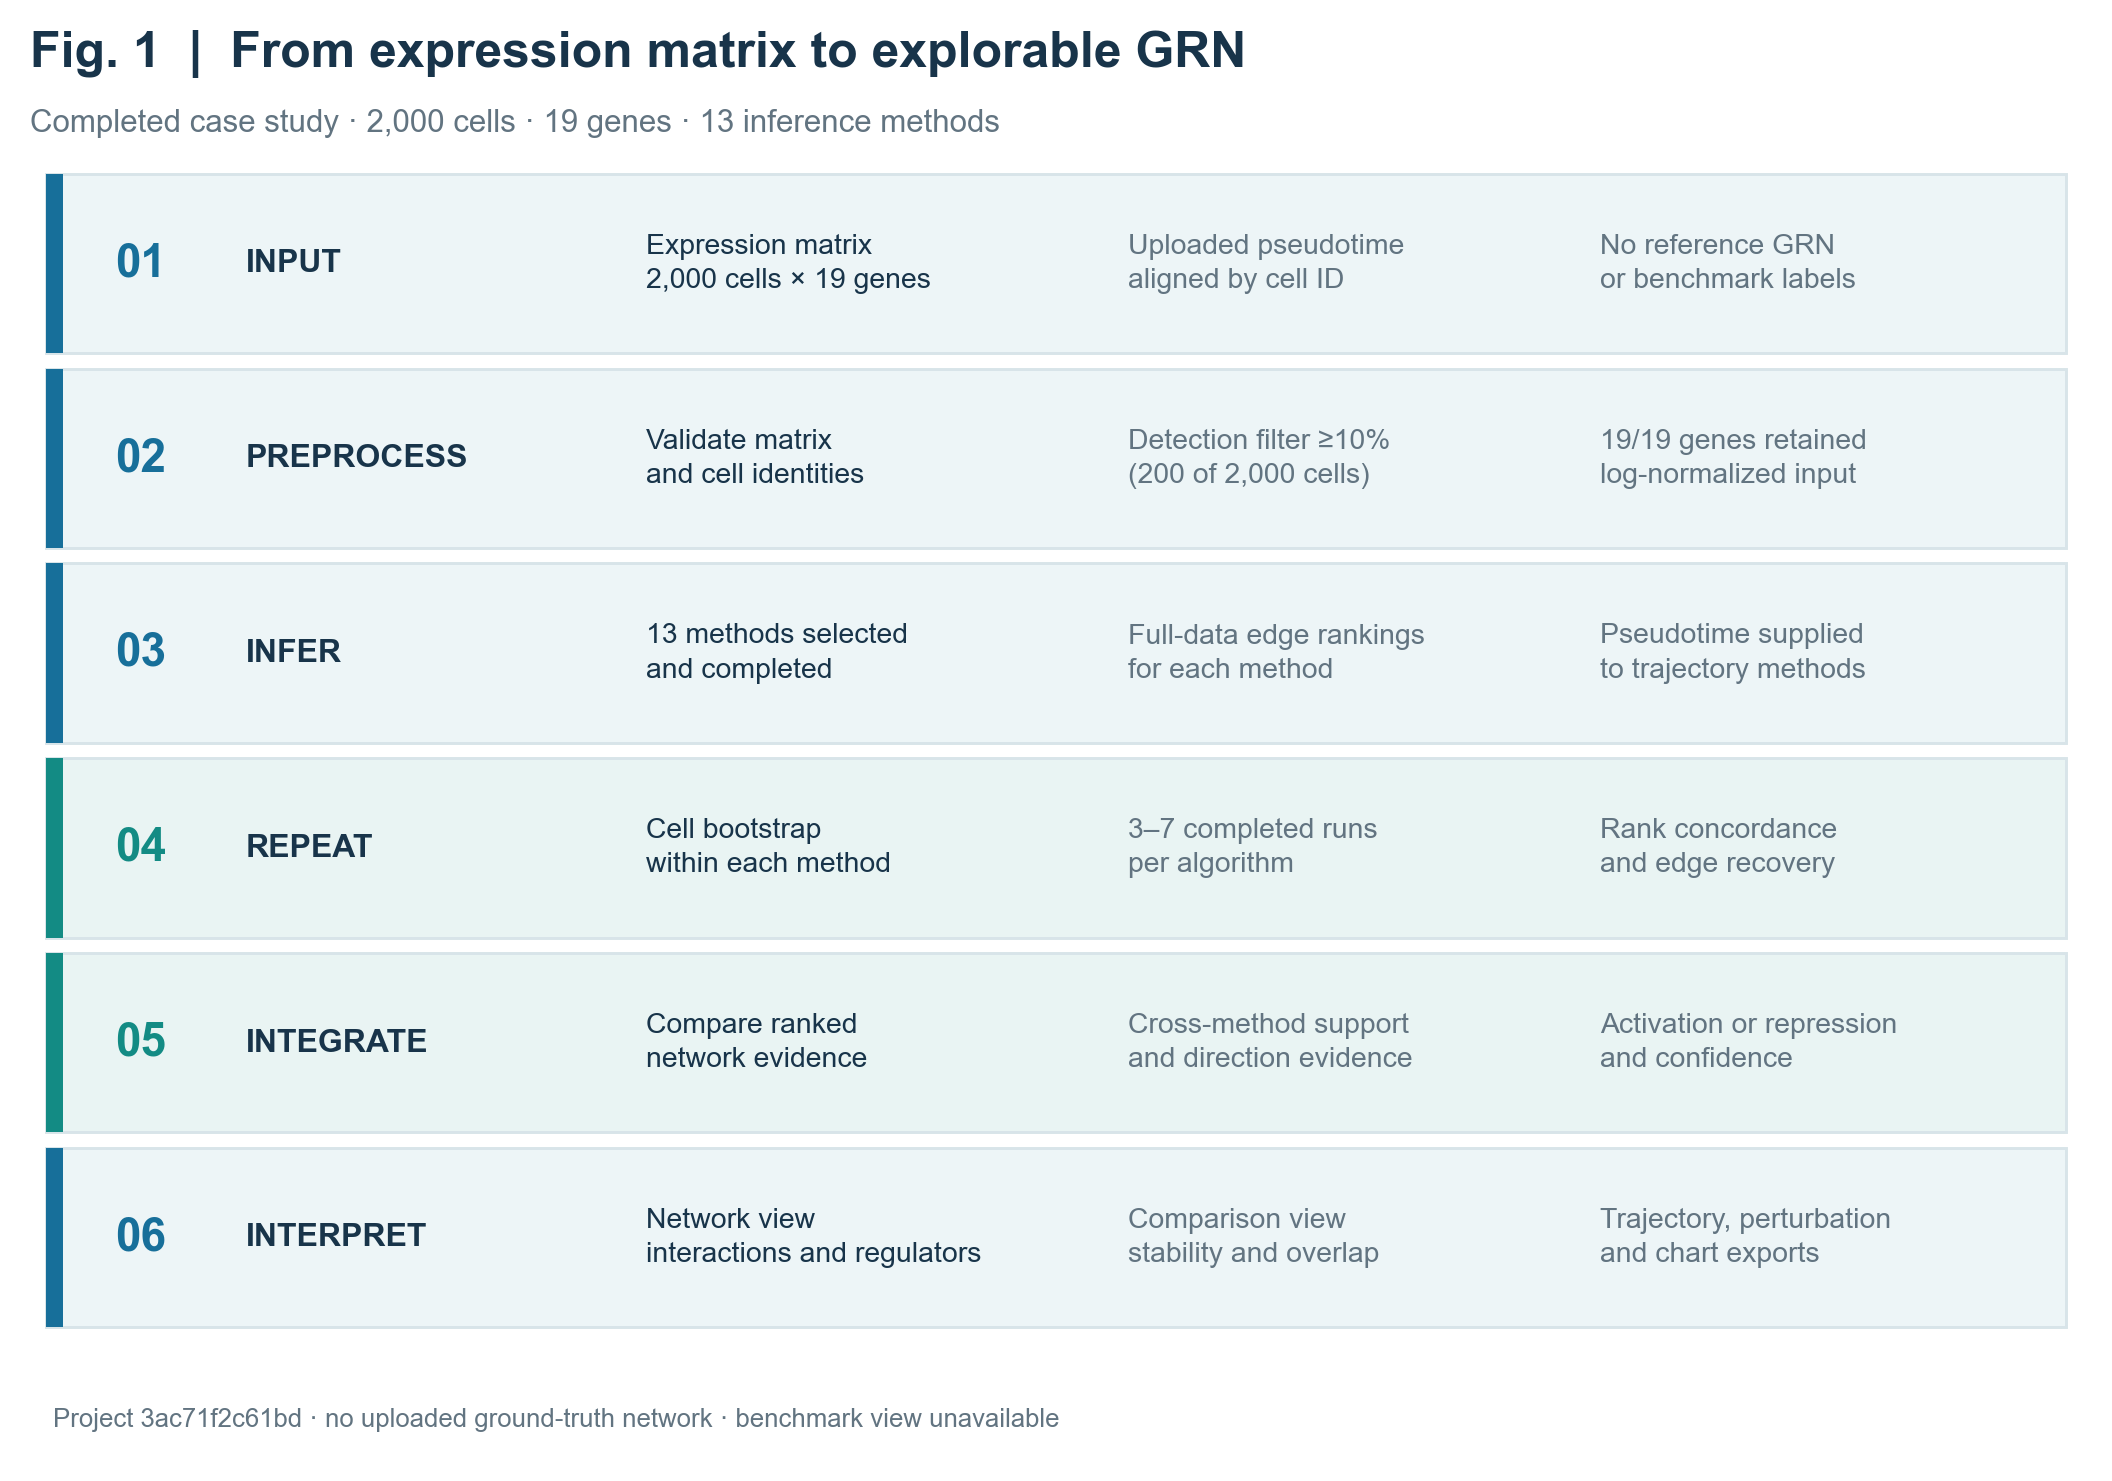
\includegraphics[width=\linewidth,height=0.68\textheight,keepaspectratio]{figure_1_detailed_workflow.png}
\caption{GRNScope analysis workflow in the completed example. The uploaded expression matrix comprised 2,000 cells and 19 genes, with supplied pseudotime and no uploaded reference network. Detection filtering at 10\% retained all 19 genes. Thirteen methods completed. Their reported bootstrap counts ranged from three to seven under automatic stopping. The final row identifies the result views available for inspection and export. The figure describes this analysis workflow; it is not a performance comparison.}
\label{fig:workflow}
\end{figure}

\begin{figure}[p]
\centering
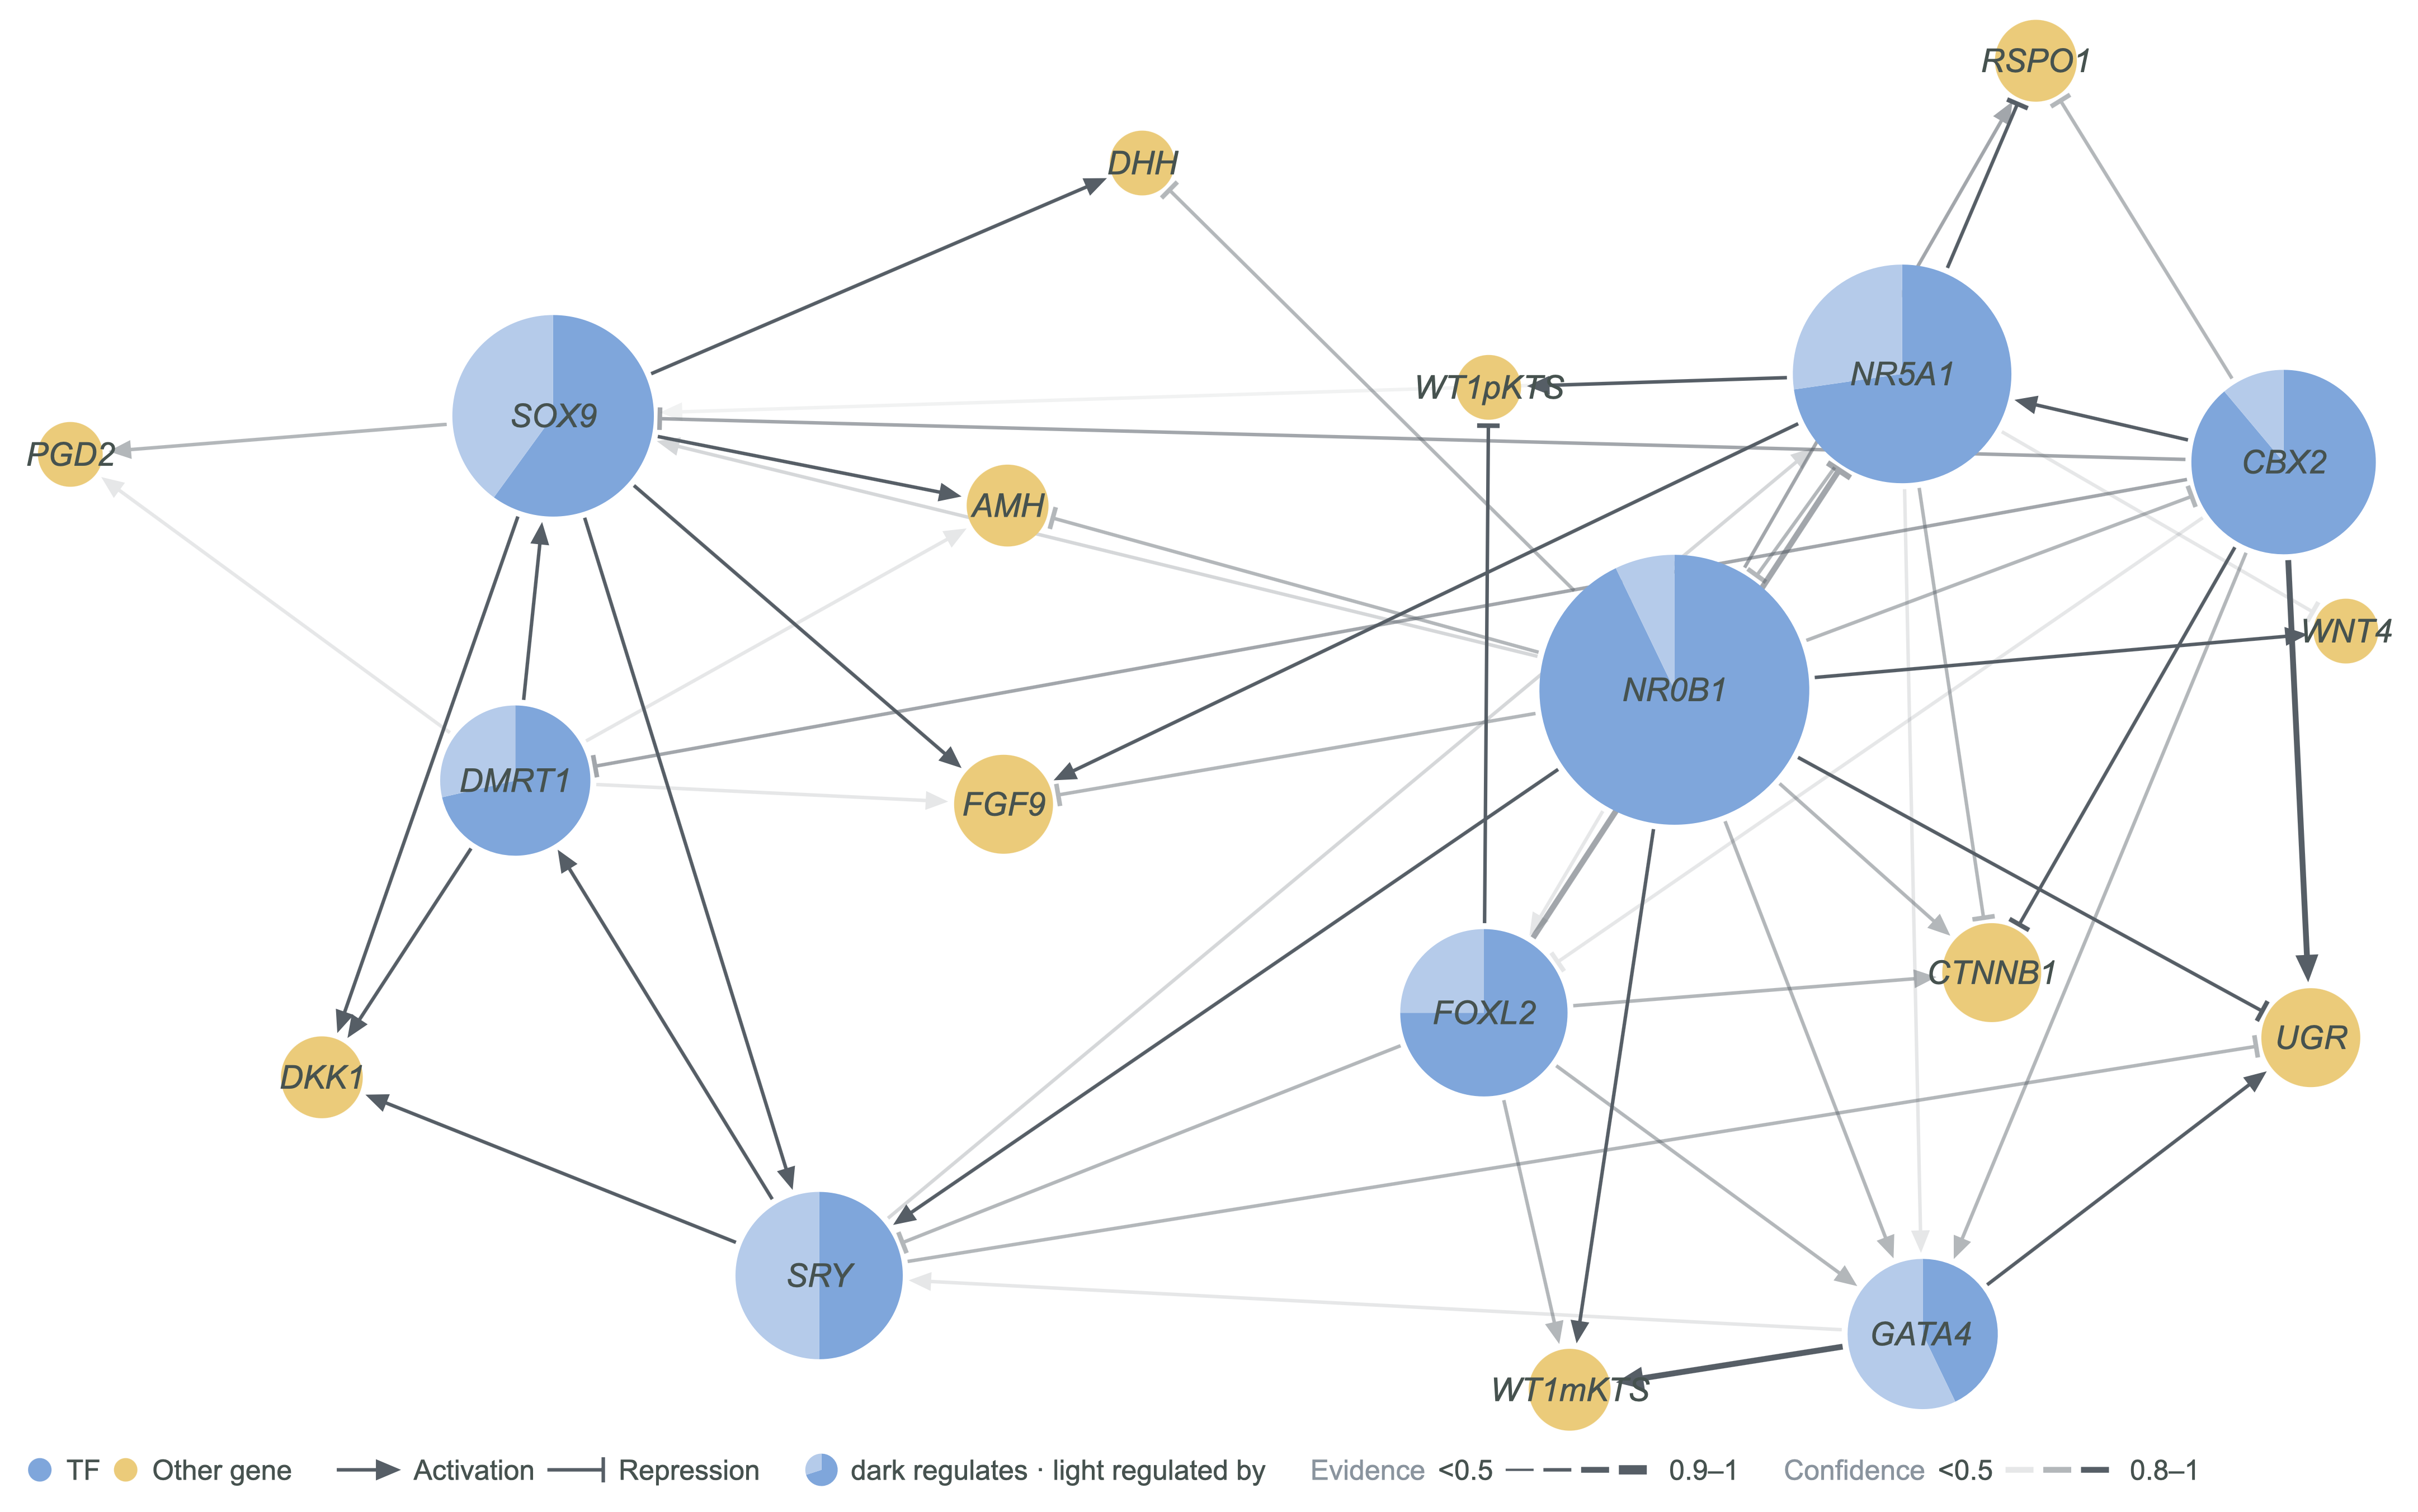
\includegraphics[width=\linewidth,height=0.68\textheight,keepaspectratio]{figure_2_website_network.png}
\caption{Predicted network exported from the GRNScope Network view. Nodes and relationships are shown under the website's selected display settings. The figure is the site's native export, including its encoding key. Direction and activation/repression marks reflect available computational evidence and should not be read as experimental validation. Only the displayed subset of relationships is shown.}
\label{fig:network}
\end{figure}

\begin{figure}[p]
\centering
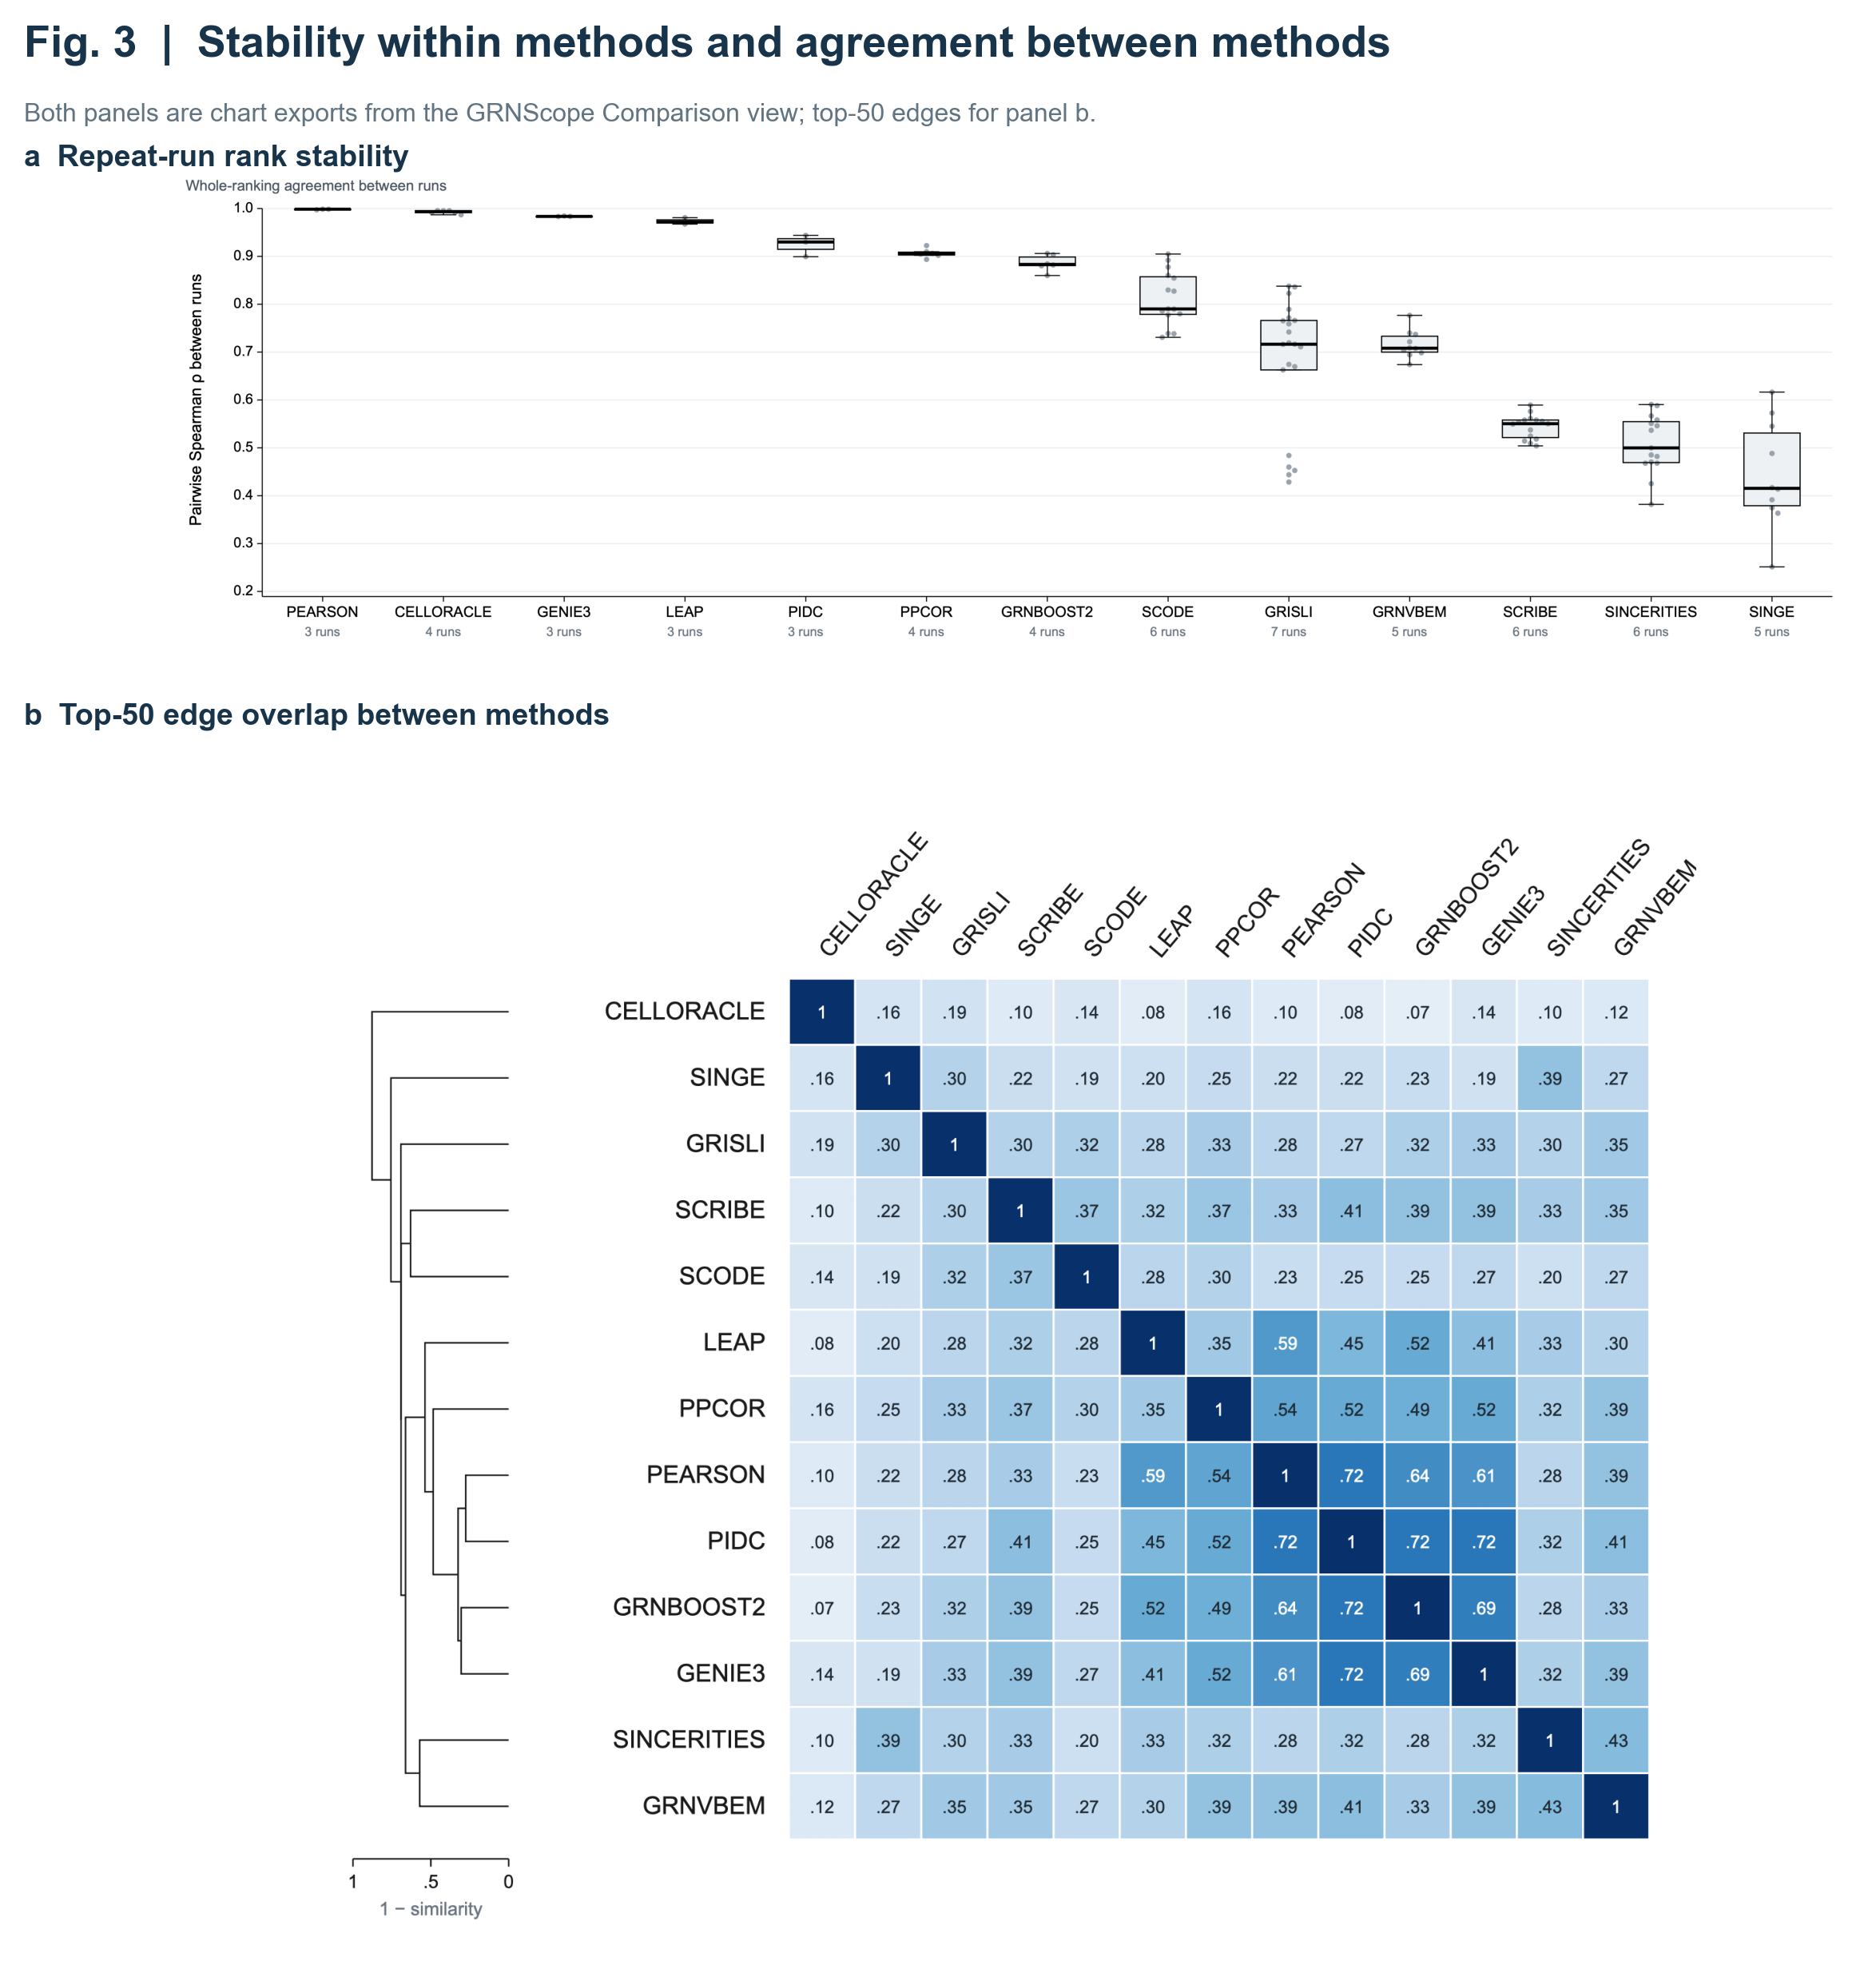
\includegraphics[width=\linewidth,height=0.68\textheight,keepaspectratio]{figure_3_website_comparison.png}
\caption{Repeat-run stability and between-method adjacency agreement. \textbf{a}, whole-ranking pairwise Spearman correlations between completed bootstrap runs within each method; run counts appear below method names. The box and points summarize observed run-pair values, not biological replicates or confidence intervals for accuracy. \textbf{b}, Jaccard similarity of each method's top 50 unique gene-pair adjacencies in the website's adjacency mode. Reverse orientations count as one adjacency. CellOracle returned fewer than 50 edges. Both panels are exports from the GRNScope Comparison view and describe reproducibility and prediction overlap, not correctness against ground truth.}
\label{fig:comparison}
\end{figure}

\clearpage

\begin{thebibliography}{9}

\bibitem{pratapa2020} Pratapa A, Jalihal AP, Law JN, Bharadwaj A, Murali TM. Benchmarking algorithms for gene regulatory network inference from single-cell transcriptomic data. \emph{Nature Methods}. 2020;17:147--154. \href{https://doi.org/10.1038/s41592-019-0690-6}{doi:10.1038/s41592-019-0690-6}.

\bibitem{chan2017} Chan TE, Stumpf MPH, Babtie AC. Gene regulatory network inference from single-cell data using multivariate information measures. \emph{Cell Systems}. 2017;5:251--267.e3. \href{https://doi.org/10.1016/j.cels.2017.08.014}{doi:10.1016/j.cels.2017.08.014}.

\bibitem{huynhthu2010} Huynh-Thu VA, Irrthum A, Wehenkel L, Geurts P. Inferring regulatory networks from gene expression data using tree-based methods. \emph{PLOS ONE}. 2010;5:e12776. \href{https://doi.org/10.1371/journal.pone.0012776}{doi:10.1371/journal.pone.0012776}.

\bibitem{moerman2019} Moerman T, Santos SA, Gonz\'{a}lez-Blas CB, et al. GRNBoost2 and Arboreto: efficient and scalable inference of gene regulatory networks. \emph{Bioinformatics}. 2019;35:2159--2161. \href{https://doi.org/10.1093/bioinformatics/bty916}{doi:10.1093/bioinformatics/bty916}.

\bibitem{kamimoto2023} Kamimoto K, Stringa B, Hoffmann CM, et al. Dissecting cell identity via network inference and in silico gene perturbation. \emph{Nature}. 2023;614:742--751. \href{https://doi.org/10.1038/s41586-022-05688-9}{doi:10.1038/s41586-022-05688-9}.

\bibitem{beeline_docs} BEELINE documentation. Reproducing BEELINE results: synthetic and curated datasets. \href{https://murali-group.github.io/Beeline/reproducing-results.html}{Project documentation}.

\end{thebibliography}

\end{document}
